\documentclass[11pt]{beamer}
\usetheme{CambridgeUS}
\usepackage[utf8]{inputenc}
\usepackage[francais]{babel}
\usepackage[T1]{fontenc}
\usepackage{amsmath}
\usepackage{amsfonts}
\usepackage{amssymb}
\usepackage{graphicx}
\usepackage{wrapfig}
\usecolortheme{beaver}
\usecolortheme[named=red]{structure}
\setbeamercolor{background canvas}{bg=gray!10!white}
\setbeamercovered{transparent} 
\setbeamertemplate{navigation symbols}{} 
\pgfdeclareimage[height=96mm,width=128mm]{ima}{mecque.png}
\setbeamertemplate{background canvas}{\pgfuseimage{ima}}
\setbeamertemplate{title page}[default][colsep=-4bp,rounded=true]

\author[ ]{L. Becquey - A. Cathignol - N. Mauvisseau - M. Simon}
\title{Feu, Bombes, et Mouvements de Foule}
\logo{
\includegraphics[scale=0.3]{logoINSA.png}} 
\institute[ ]{INSA de Lyon\\ Bio-Informatique et Modélisation} 
\date{Projet 3BIM 2015-2016} 
\subject{Projet 3BIM} 
\AtBeginSection[]{
  \begin{frame}
    \frametitle{Feu, Bombes, et Mouvements de Foule}
    \tableofcontents[currentsection]
  \end{frame}
}

\begin{document}

\begin{frame}
\titlepage
\end{frame}
\setbeamertemplate{background canvas}[default]


\section{Objectifs}

\begin{frame}{La Démarche}
\begin{alertblock}{Le problème}
\footnotesize
\textit{Comment prévoir, anticiper et minimiser les conséquences de mouvements de foule dans différentes conditions extrêmes (non réalisables en pratique) pour un bâtiment donné ?}
\end{alertblock}
\begin{exampleblock}{Le défi}
\footnotesize
\textbf{Construire une simulation réaliste des mouvements de foule dans un bâtiment donné.}
\end{exampleblock}
\begin{itemize}
\item \textbf{Récolte d'informations:} accumuler des données sur le comportement réel des foules d'après des articles scientifiques
\item \textbf{Construction du modèle:} Inclure ces informations sur le comportement dans une simulation numérique
\item \textbf{Estimer:} en mesurant et observant les résultats de la simulation
\item \textbf{Conclure:} quand à la sécurité du bâtiment
\end{itemize}
\end{frame}
\section{Exemple d'informations récoltées}

\begin{frame}{Exemple d'informations récoltées}
La lecture d'articles scientifiques permet d'obtenir des donnés chiffrées, par exemple:
\begin{wrapfigure}[10]{l}{2.5cm}
	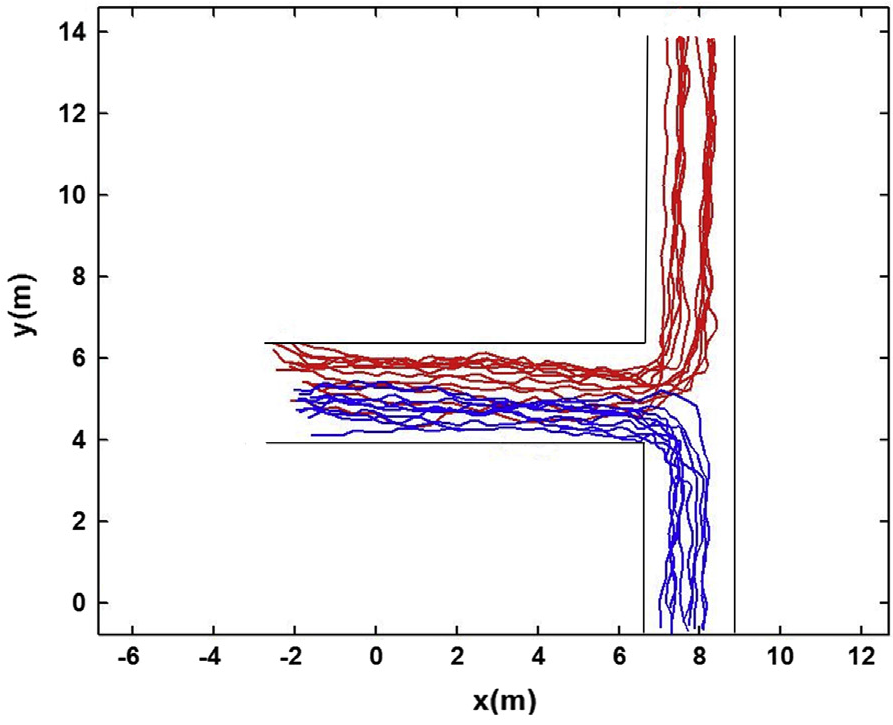
\includegraphics[scale=0.1]{T.png}
	\caption{\tiny Exemple d'étude réalisée sur les couloirs en T}
\end{wrapfigure}
\begin{itemize}
\item Il existe une vitesse idéale pour la fluidité du mouvement, vers laquelle tendent les vitesses des piétons après une perturbation
\item Ralentissement de 34\% lors de la rencontre de deux flux de piétons dans un "T"
\item Différences de comportement en état normal ou état de stress
\end{itemize}
\end{frame}


\section{Choix}
    \subsection{Restrictions}
    
\begin{frame}{Restrictions}
\begin{itemize}
\item On utilise des bâtiments simples, rectangulaires \textit{(et à murs perpendiculaires)}
\item On ne considère qu'un seul étage à la fois
\end{itemize}
\end{frame}

    \subsection{Hypothèses du modèle}
    
\begin{frame}{Hypothèses du modèle}
\begin{block}{Différents moteurs physiques à essayer}
\begin{itemize}
\item Obstacle: Je m'arrête
\item Obstacle: Je me décale
\item Obstacle: Si trop de pression derrière, je bouscule
\end{itemize}
\end{block}

\begin{block}{L'idée: phénomène d'emportement}
$$\textrm{mouvement} = \frac{( \alpha . \textrm{volonté du piéton} + (1-\alpha) \textrm{ volonté de la foule} )}{2}$$
\vspace{0.5cm}
\end{block}
$\alpha$ varie selon l'humeur et l'état de stress du piéton.
\end{frame}

\section{Le Modèle}
    \subsection{Le bâtiment}

\begin{frame}{Modèle de bâtiment}

\begin{wrapfigure}[1]{r}{2.5cm}
	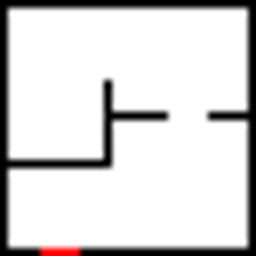
\includegraphics[scale=0.2]{little-room.png}
	\caption{\tiny Image d'entrée modélisant un étage.}
\end{wrapfigure}

\textit{On utilise des plans d'étage avec des murs en noir sur fond blanc comme support d'entrée.}\\
Un ou plusieurs accès par bâtiment sont possibles.\\
\vspace{0.5cm}
\textbf{\large Modélisation:}
\begin{itemize}
\item Attributs de dimensions \textit{(fixes)}
\item Grille booléenne de 0 \textit{(pas de mur)} ou 1 \textit{(mur)}
\item Liste de piétons présents à l'intérieur
\end{itemize}
\end{frame}    
    
\begin{frame}{Modéliser un étage avec la théorie des Graphes}
La topographie intérieure peut se modéliser comme une succession de \textbf{nœuds} \textit{(points de rencontre, croisements)} et \textbf{segments} \textit{(couloirs)}.\\

\begin{block}{Assigner chaque zone à un nœud:}
\hspace{1cm}
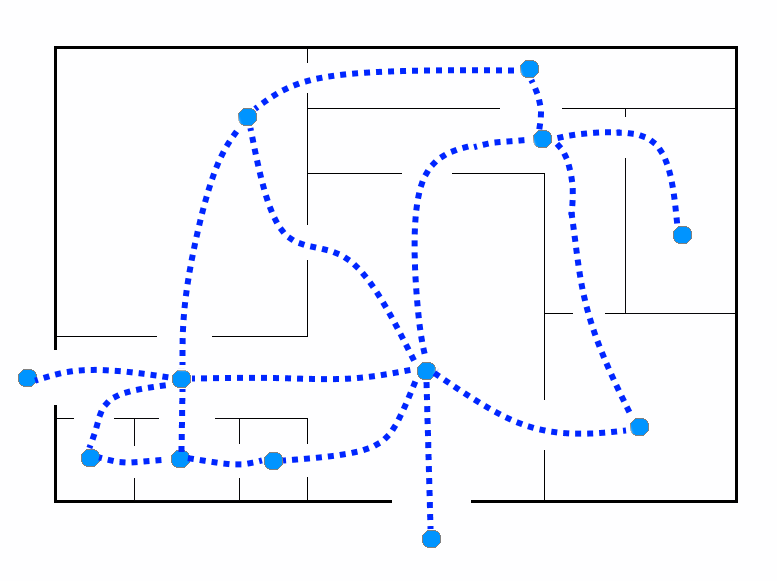
\includegraphics[scale=0.2]{noeuds.png}
\hspace{1cm}
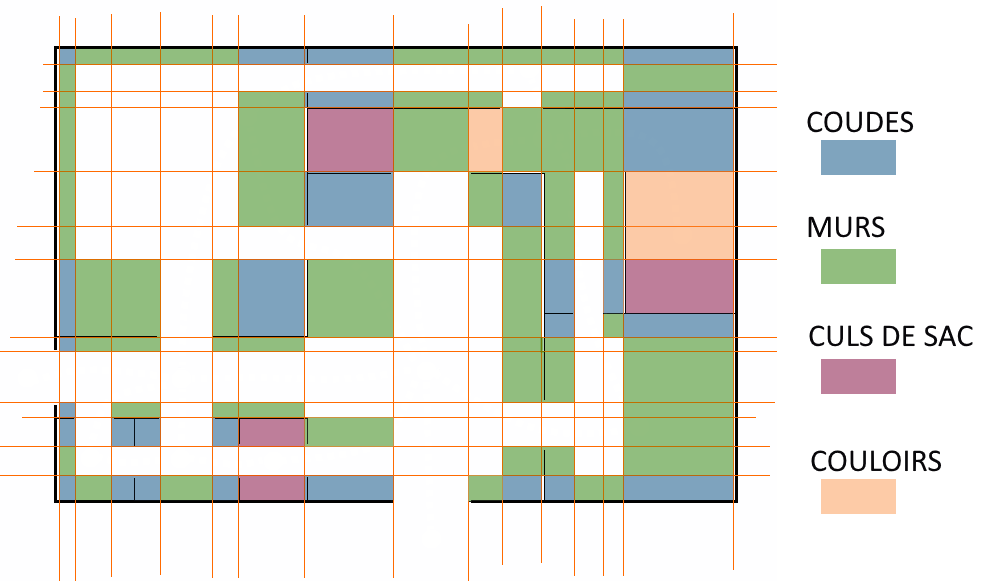
\includegraphics[scale=0.2]{carres.png}
\end{block}

\textbf{MAIS} On souhaite conserver la \textbf{largeur} ! $\Rightarrow$ Associer une zone à un nœud "rectangulaire".\\

\textbf{Chaque rectangle est un nœud en relation avec $\leq 4$ autres.}
\vspace{0.5cm}
\end{frame}
    
    \subsection{L'individu}
    
\begin{frame}{Modèle d'individu}
\textit{Les  piétons existent à des coordonnées flottantes, et ne sont pas limités à un "case".}\\
$\Rightarrow$ une \textbf{densité} de population est donc définie sur chaque case.\\
\vspace{0.5cm}
\textbf{\large Modélisation:}
\begin{itemize}
\item \textbf{Attributs de position} flottants, aléatoires ou non \textit{(x et y)}
\item \textbf{Rayon de la personne}, aléatoire \textit{(La place qu'elle occupe)}
\item \textbf{Vecteur vitesse} et \textbf{vecteur accélération}
\item Liste ordonnée de points \textit{(la trajectoire que le piéton} \textbf{souhaite suivre})
\item Attribut d'\textbf{humeur}, pour varier le comportement \textit{(état de stress)}
\end{itemize}
\end{frame}


    \subsection{La population}

\begin{frame}{Modèle de population}
\textit{La population représente la tendance moyenne du groupe de piétons.}\\
\vspace{0.5cm}
\textbf{\large Modélisation:}
\begin{itemize}
\item \textbf{Vecteur vitesse} et \textbf{vecteur accélération}\\
$\Rightarrow$ Moyenne des directions unitaires\\
$\Rightarrow$ Médiane des normes \textit{(Moins sensible aux extrêmes)}
\item Seuil de densité limite \textit{(à partir duquel il y a des morts ou des piétinés)}
\end{itemize}
\end{frame}

\section{Vérification du modèle}
\begin{frame}{Régression ?}
Il faudrait comparer des données réelles aux mesures numériques pour valider le modèle.
\end{frame}

\section{Mesures}
\begin{frame}{Mise à l'épreuve d'un bâtiment réel}
On peut ainsi soumettre les plans du nouveau bâtiment de Génie Mécanique de l'INSA à notre simulation.\\
\vspace{1cm}

En fonction des résultats, on pourra conclure quand à la validité des normes européennes, ou, à défaut, démolir le nouveau bâtiment de l'INSA.
\end{frame}

\section{Réferences}
\begin{frame}{Références}[allowframebreaks]
\footnotesize
    
  \begin{thebibliography}{10}    
  \beamertemplatebookbibitems
  
  \bibitem{Autor1990}
    A.~Autor.
    \newblock {\em Introduction to Giving Presentations}.
    \newblock Klein-Verlag, 1990.

  \beamertemplatearticlebibitems

  \bibitem{Jemand2000}
    S.~Jemand.
    \newblock On this and that.
    \newblock {\em Journal of This and That}, 2(1):50--100, 2000.

  \end{thebibliography}
\end{frame}

\end{document}